%; whizzy chapter
% -initex iniptex -latex platex -format platex -bibtex jbibtex -fmt fmt
% $B0J>e(B whizzytex $B$r;HMQ$9$k>l9g$N@_Dj!#(B


%     Tokyo Debian Meeting resources
%     Copyright (C) 2008 Junichi Uekawa
%     Copyright (C) 2008 Nobuhiro Iwamatsu

%     This program is free software; you can redistribute it and/or modify
%     it under the terms of the GNU General Public License as published by
%     the Free Software Foundation; either version 2 of the License, or
%     (at your option) any later version.

%     This program is distributed in the hope that it will be useful,
%     but WITHOUT ANY WARRANTY; without even the implied warranty of
%     MERCHANTABILITY or FITNESS FOR A PARTICULAR PURPOSE.  See the
%     GNU General Public License for more details.

%     You should have received a copy of the GNU General Public License
%     along with this program; if not, write to the Free Software
%     Foundation, Inc., 51 Franklin St, Fifth Floor, Boston, MA  02110-1301 USA

%  preview (shell-command (concat "evince " (replace-regexp-in-string "tex$" "pdf"(buffer-file-name)) "&"))
% $B2hA|%U%!%$%k$r=hM}$9$k$?$a$K$O(Bebb$B$rMxMQ$7$F(Bboundingbox$B$r:n@.!#(B
%(shell-command "cd image200804; ebb *.png")

%%$B$3$3$+$i%X%C%@3+;O!#(B

\documentclass[mingoth,a4paper]{jsarticle}
\usepackage{monthlyreport}
\usepackage[dvips]{xy}

% $BF|IU$rDj5A$9$k!"Kh7nJQ$o$j$^$9!#(B
\newcommand{\debmtgyear}{2008}
\newcommand{\debmtgmonth}{7}
\newcommand{\debmtgdate}{19}
\newcommand{\debmtgnumber}{42}

\begin{document}

\begin{titlepage}
\thispagestyle{empty}

% $B%?%$%H%k%Z!<%8(B:$BJT=8I,MW$JItJ,$O:G=i$N%^%/%m$KHt$P$9$3$H(B

\vspace*{-2cm}
$BBh(B\debmtgnumber{}$B2s(B $BEl5~%(%j%"(B Debian $BJY6/2q;qNA(B

\hspace*{-2.4cm}
\includegraphics[width=210mm]{image200801/2008title.eps}\\
\hfill{}\debmtgyear{}$BG/(B\debmtgmonth{}$B7n(B\debmtgdate{}$BF|(B

\end{titlepage}

\dancersection{Introduction}{$B>e@n(B $B=c0l(B}
 
 $B:#7n$N(BDebian$BJY6/2q$X$h$&$3$=!#$3$l$+$i(BDebian$B$N@$3&$K$"$7$rF'$_F~$l$k$H(B
 $B$$$&J}$b!"$9$G$K$I$C$W$j$H$D$+$C$F$$$k$H$$$&J}$b!"7n$K0l2s(BDebian$B$K$D$$(B
 $B$F8l$j$^$;$s$+!)(B

 Debian$BJY6/2q$NL\E*$O2<5-$G$9!#(B

\begin{itemize}
 \item \underline{Debian Developer} ($B3+H/<T(B)$B$N0i@.!#(B
 \item $BF|K\8l$G$N!V(B\underline{$B3+H/$K4X$9$k>pJs(B}$B!W$r@0M}$7$F$^$H$a!"%"%C%W%G!<%H$9$k!#(B
 \item \underline{$B>l(B}$B$NDs6!!#(B
 \begin{itemize}
  \item $BIaCJ$P$i$P$i$J>l=j$K$$$k?M!9$,(B face-to-face $B$G=P2q$($k>l$rDs6!(B
	$B$9$k!#(B
  \item Debian $B$N$?$a$K$J$k$3$H$r8l$k>l$rDs6!$9$k!#(B
  \item Debian$B$K$D$$$F8l$k>l$rDs6!$9$k!#(B
 \end{itemize}
\end{itemize}		

 Debian$B$NJY6/2q$H$$$&$3$H$G5f6KE*$K$O;22C<TA40w$,(BDebian Package$B$r$,$j$,$j(B
 $B$H:n$k%9!<%Q!<%O%C%+!<$K$J$C$?;Q$rLQA[$7$F$$$^$9!#>pJs$N6&M-!&3hMQ$rDL$7(B
 $B$F(B Debian$B$N:#8e$NG=F0E*$JE83+$X$NEZBf$H$7$F!"!V>l!W$H$7$F$N6u4V$rDs6!$9(B
 $B$k$N$,L\E*$G$9!#(B

$B0J>e$rL\E*$H$7$?!"(B2008 $BG/%"%8%'%s%@$G$9!'(B
\begin{enumerate}
 \item $B?7G/2q!V5$9g$rF~$l$k!W(B
 \item Open Source Conference Tokyo (3/1)
 \item $B%G!<%?$@$1$N%Q%C%1!<%8$r:n@.$7$F$_$k!"(B
       $B%i%$%;%s%9$N9M$(J}(B (David Smith)
 \item $B%P%$%J%j0l$D$N%Q%C%1!<%8$r:n@.$7$F$_$k(B ($B5HED(B@$BHD66(B)\\
       $B%P!<%8%g%s4IM}%D!<%k$r;H$$(BDebian$B%Q%C%1!<%8$r4IM}$9$k(B(git)\\
       $B%"%C%W%9%H%j!<%`$N07$$(B(svn/git/cvs)($B4d>>(B $B?.MN$5$s(B)
 \item $B%P%$%J%j$NJ,$1$?%Q%C%1!<%8$N:n@.!#(B($BA0ED$5$s(B)\\
       $B%P%$%J%j$NJ,$1J}$N9M$(J}!"%"%C%W%0%l!<%I$J$I$N1?MQ$H$+!#(B
 \item $B%Q%C%1!<%8:n@.(B(dpatch/debhelper$B$G:n@.$9$k%Q%C%1!<%8(B)($B>.NS576)$5$s(B)\\
       man $B$N=q$-J}(B(roff or docbook)($B$G$s$5$s(B)
       OSC 2008 Hokkaido
 \item $B%Q%C%1!<%8:n@.(B(kernel patch$B!"(Bkernel module)($B4d>>(B $B?.MN(B)
       Debconf$BH/I=N}=,!J>e@n$5$s!K(B

 \item Debconf $B%"%k%<%s%A%s!"6&M-%i%$%V%i%j%Q%C%1!<%8:n@.(B
       $B%3%_%C%/%^!<%1%C%H(B74

 \item Open Source Conference Tokyo/Fall$B!"(B
       $B%G!<%b%s7O$N%Q%C%1!<%8$N:n@.!"(Blatex$B!"(B emacs-lisp$B!"%U%)%s%H%Q%C%1!<%8(B
 \item $B%Q%C%1!<%8$N(B cross-compile $B$NJ}K!!"(Bamd64 $B>e$G(B i386 $B$N%Q%C%1!<%8$H(B
       $B$+!"(BOSC-Fall$BJs9p2q!"(BDebconf$BJs9p2q(B
 \item $B9q:]2=(B po-debconf / po$B2=(B / DDTP
 \item $BK:G/2q(B
\end{enumerate}


\newpage

\begin{minipage}[b]{0.2\hsize}
 \definecolor{titleback}{gray}{0.9}
 \colorbox{titleback}{\rotatebox{90}{\fontsize{80}{80} {\gt $B%G%S%"%sJY6/2q(B} }}
\end{minipage}
\begin{minipage}[b]{0.8\hsize}
\hrule
\vspace{2mm}
\hrule
\tableofcontents
\vspace{2mm}
\hrule
\end{minipage}

\dancersection{$B;vA02]Bj(B}{$B4d>>(B $B?.MN(B}

$B:#2s$N;vA02]Bj$O0J2<$G$9!#(B

\begin{enumerate}
 \item ...

\end{enumerate}

$B$3$N2]Bj$KBP$7$FDs=P$$$?$@$$$?FbMF$O0J2<$G$9!#(B


%%% trivia quiz
\dancersection{Debian Trivia Quiz}{$B>.NS(B $B576)(B}

$B$H$3$m$G!"$_$J$5$s(B Debian $B4XO"$NOCBj$K$*$$$D$$$F$$$^$9$+!)(BDebian$B4XO"$NOC(B
$BBj$O%a!<%j%s%0%j%9%H$r$h$s$G$$$k$HDI@W$G$-$^$9!#$?$@$h$s$G$$$k$@$1$G$O$O(B
$B$j$"$$$,$J$$$N$G!"M}2rEY$N%F%9%H$r$7$^$9!#FC$K0l?M$@$1$G$O0UL#$,$o$+$i$J(B
$B$$$H$3$m$b$"$k$+$bCN$l$^$;$s!#$_$s$J$G0l=o$KFI$s$G$_$^$7$g$&!#(B

$B:#2s$N=PBjHO0O$O(B\url{debian-devel-announce@lists.deban.org} $B$KEj9F$5$l$?(B
$BFbMF$H(BDebian Project News$B$+$i$G$9!#(B
% $B=PBjHO0O(B: http://lists.debian.org/debian-devel-announce/2008/06/msg00004.html $B!A(B http://lists.debian.org/debian-devel-announce/2008/07/msg00004.html
\begin{multicols}{2}
 \subsection{debian-devel-announce}
 \url{debian-devel-announce@lists.deban.org}$B$X$NEj9FFbMF$+$i$G$9!#(B
 
 \santaku
 {Perl 5.10$B$N%P%0$G$I$N$h$&$JLdBj$,H/@8$7$?(B?}
 {Ruby$B$H(BPython$B$G=q$+$l$?%"%W%j%1!<%7%g%s$d%i%$%V%i%j$,%$%s%9%H!<%k$G$-$J$$(B}
 {$B%$%s%9%H!<%k$5$l$?%U%!%$%k$N%Q!<%_%C%7%g%s$,(B0777$B$K$J$k(B}
 {$BFCDj$NL>A0$N%U%!%$%k$,%$%s%9%H!<%k$G$-$J$$(B}
 {B}% File::Path::rmtree$B$,%D%j!<:o=|A0$K%Q!<%_%C%7%g%s$r(B0777$B$K$7!"$=$l$,(Bsymlink$B$N%j%s%/85$K$bEAGE$9$k$h$&$K$J$C$F$$$?$N$,860x!#(Bpostinst$B$G8F$S=P$5$l$k(Bdebsign$B$,%D%j!<$N(Bsymlink$B$r:n@.$7$F%O%C%7%e$r7W;;$7$?8e!"$3$N4X?t$r;H$C$F(Bsymlink$B$r:o=|$7$F$$$k$N$G!"%$%s%9%H!<%k8e$K%U%!%$%k$N%Q!<%_%C%7%g%s$,=q$-49$($i$l$kLdBj$KH/E8$7$?(B
 
 \santaku
 {Debian$B%W%m%8%'%/%HFb$N%A!<%`$K4X$9$kD4::$GH=L@$7$?!VM=A[30$N%A!<%`!W$G$J$$$b$N$O(B?}% $BD4::$O(BDPL$B$N(BSteve McIntyre$B$,9T$C$F$$$k(B
 {$B<B:]$KF0$$$F$$$k$N$O(B1$B?M$@$1$H$$$&%A!<%`(B}
 {$BC/$,:n6H$9$k$+Kh2s$8$c$s$1$s$G7h$a$F$$$k%A!<%`(B}
 {$B$*4j$$$d$"$j$,$H$&$G$O$J$/6<Gw$GF0$$$F$$$k%A!<%`(B}
 {B}
 
 \santaku
 {wxwidgets2.8$B$,%"%C%W%m!<%I$5$l$?$,!"D9$$$3$H(Bwxwidgets2.6$B$N;~Be$,B3$$$F$$$?!#$=$NM}M3$O(B?}
 {$B%Q%C%1!<%8%a%s%F%J$,J]<iE*$G!"(B2.8$B$N;HMQ$KBP$7$FHs@Q6KE*$@$C$?(B}
 {$B%"%C%W%m!<%I$7$?$H$3$m$G$I$&$;C/$b;H$C$F$/$l$J$$$H%Q%C%1!<%8%a%s%F%J$,;W$C$?(B}
 {$B%Q%C%1!<%8%a%s%F%J$,B?K;$G:n6H;~4V$,$H$l$J$+$C$?(B}
 {A}% lenny$B$G$O(B2.6$B$r%G%U%)%k%H$H$7!"(B2.6$B$GF0$+$J$$$b$N$@$1(B2.8$B$r;H$C$F$[$7$$!"$H$N$3$H(B
 
 \santaku
 {Frans Pop$B$N<-G$$K$h$C$F!"?7$?$J<9I.<T$,5a$a$i$l$k$h$&$K$J$C$?$b$N$H$O(B?}
 {$B%j%j!<%9%N!<%H(B}
 {Debian Project Blog}% Debian Project$B8x<0$N(Bblog
 {DEB NOTE}% $BL>A0$,=q$+$l$?3+H/<T$r6/@)E*$K%3%_%e%K%F%#$+$iDI$$=P$9%N!<%H(B
 {A}
 
 \subsection{Debian Project News 2008$BG/(B05$B9f(B}
 \url{http://www.debian.org/News/weekly/2008/05/}
 $B$K$"$k(B6$B7n(B23$BF|HG$G$9!#(B
 
 \santaku
 {debian/rules$B$N(Bget-orig-source$B%?!<%2%C%H$O2?$r5-=R$9$k$?$a$N$b$N$+(B?}
 {$B!V%*%j%8!{J[Ev!W$GJ[Ev$K%=!<%9$r$D$1$F$b$i$&J}K!(B}
 {upstream$B$+$i%M%C%H%o!<%/7PM3$G%=!<%9%3!<%I$r<hF@$7$F8=:_$N%=!<%9%3!<%I$HCV$-49$($kJ}K!(B}
 {upstream$B$+$i%M%C%H%o!<%/7PM3$G:G?7$N(B.orig.tar.gz$B%U%!%$%k$r<hF@$9$kJ}K!(B}
 {C}% $B$"$^$j=q$+$l$k$3$H$N$J$$%?!<%2%C%H$@$,!"(Bskkdic$B$G$O(BCVS$B7PM3$G<hF@$9$k$h$&@_Dj$7$F$$$k(B
 
 \santaku
 {$B%j%j!<%9%4!<%k$K4X$9$k(BPeter Eisentraut$B$N0U8+$O(B?}
 {$B%j%j!<%9%4!<%k$J$s$F=jA'0lIt$N3+H/<T$N3Z$7$_$K2a$.$J$$(B}
 {Debian$B$N5!G=$N<BAu$K4X$9$k%j%j!<%9%4!<%k$O%j%j!<%98e$K%]%j%7!<$X$HJQ$($k$Y$-$@(B}
 {$B%j%j!<%9$J$s$F>~$j$G$9!#0N$$?M$K$O$=$l$,$o$+$i$s$N$G$9$h(B}
 {B}
 
 \santaku
 {William Pitcock$B$,:o=|$rDs0F$7$?%V!<%H%m!<%@%Q%C%1!<%8$O(B?}
 {grub}
 {lilo}
 {yaboot}
 {B}% $B4JC1$K$OD>$;$J$$(Bgrave$B$J%P%0$,$"$k(B
 
 \santaku
 {Debian weather$B$H$O$I$s$J%5!<%S%9$+(B?}
 {$BFCDj%"!<%-%F%/%A%c$N%"!<%+%$%V$N>uBV$rMWLs$7$FI=<($9$k(B}% $B$=$NI=<($KE75$$N5-9f$r;HMQ$7$F$$$k(B
 {Debian$B4XO"%[%9%H$,CV$+$l$F$$$k@$3&3FCO$NE75$$rI=<($9$k(B}% worldwide$B$GF/$$$F$$$k$H$$$&0U<1$r9b$a$k(B
 {$B%a!<%j%s%0%j%9%H$NN.NL$+$i@$3&3FCO$NE75$$r?dB,$7$FI=<($9$k(B}% $B$3$NCO0h$+$i$N%a!<%k$,B?$$$+$i$3$NCO0h$O1+$@$J!"$H$+(B
 {A}
 
 \subsection{Debian Project News 2008$BG/(B06$B9f(B}
 \url{http://www.debian.org/News/weekly/2008/06/}
 $B$K$"$k(B7$B7n(B7$BF|HG$G$9!#(B
 
 \santaku
 {Debian 15$B<~G/$O$$$D$+(B?}
 {$B<!2s$NEl5~%(%j%"(BDebian$BJY6/2q3+:EM=DjF|$G$"$k(B8$B7n(B16$BF|(B}
 {$BK\F|(B7$B7n(B19$BF|(B}
 {$B5c$/;R$bL[$k(B7$B7n(B9$BF|(B}
 {A}
 
 \santaku
 {Debian$B$N%a%K%e!<(B (.menu$B%U%!%$%k(B) $B$H%G%9%/%H%C%W4D6-$N%a%K%e!<(B (.desktop$B%U%!%$%k(B) $B$K4X$9$k5DO@$O$I$N$h$&$J7kO@$KMn$ACe$$$?$+(B?}
 {freedesktop.org$B$N(B.desktop$B%U%!%$%k$r(BDebian$B$K9g$&$h$&3HD%$7$F;H$C$F$$$3$&(B}
 {freedesktop.org$B$N(B.desktop$B%U%!%$%k$K$OITJX$JE@$,$"$k$N$G!"F/$-$+$1$F=$@5$7$F$b$i$*$&(B}
 {freedesktop.org$B$N(B.desktop$B%U%!%$%k$O;H$($J$$$N$G(BDebian$B$N(B.menu$B%U%!%$%k$r;H$o$;$h$&(B}
 {A}% .desktop$B%a%K%e!<$O%f!<%6%S%j%F%#$rL\E*$H$9$k$b$N$GC10l3,AX(B ($B%5%V%+%F%4%j$J$7(B) $B$J$N$KBP$7!"(BDebian$B$N%a%K%e!<$O40A4@-$rL\E*$H$9$k$b$N$G3,AX$r?<$/7!$C$F$$$k!#$A$J$_$K(B.menu$B$KHf$Y$F(B.desktop$B$N$[$&$,$$$$$H$$$&?M$O$+$J$jB?$=$&(B
 
 \santaku
 {6$B7nKv$K=i$a$FCB@8$7$?(BDebian$B3+H/<TF1;N$NIWIX$H$O(B?}
 {Junichi Uekawa$B$H(BKenshi Muto}
 {Meike Reichle$B$H(BAlexander Schmehl}
 {Debra Murdock$B$H(BIan Murdock}% $B<B$O(BDebra$B$5$s$,(BDD$B$K$J$j:#99$J$,$i7k:'!"$H$+(B
 {B}
 
 \santaku
 {$B7k:'$7$?Fs?M$K$D$$$F=R$Y$?0J2<$N;v9`$N$&$A!"@5$7$$$b$N$O(B?}
 {$B:G=i$NB#$jJ*(B: DebConf5$B$NEZ;:(B}% $B6qBNE*$K$O(BDebConf5$B$N(BT$B%7%c%D$H%U%#%s%i%s%I$N%A%g%3%l!<%H(B
 {$BHkL)$N0&$N8r49<jCJ(B: wiki.debian.org}% planet.d.o$B$G8r49$7$F$$$?$iC/$+$K=q$-49$($i$l$?(B
 {$B:'Ls$N8x<0H/I=<jCJ(B: lists.debian.org}% planet.d.o$B$GH/I=$7$?$iL>A0$r=q$-49$($i$l$?(B
 {A}

\end{multicols}

\dancersection{$B:G6a$N(BDebian$B4XO"$N%_!<%F%#%s%0Js9p(B}{$B>e@n(B $B=c0l(B}
\subsection{$BEl5~%(%j%"(BDebian$BJY6/2q(B41$B2sL\Js9p(B}

% (query-replace-regexp "<.*?>" "")
% (query-replace-regexp "^[	 ]\+" "")


\subsection{eeePC Developers Conference day 1}

$B7P:QIt9)6H6I!#(B
$BEPO?$7$?$iL5NA$G;22C$G$-$k%+%s%U%!%l%s%9!#(B
$B9V1i<T$,A40w%9!<%D$r$-$F$$$^$9$,!"Mh>l$7$F$$$kJ}!9$OIaCJCe$G$9!#(B
$B%+%a%i$N%U%i%C%7%e$NNL$+$i$OCmL\EY$,;G$($^$9!#(B
$B7HBSEEOC$NCe?.2;$,$J$j$[$&$@$$$G$9!#(B

$B3+;O$N%*!<%W%K%s%0$OB?>/$*$/$l$^$7$?$,$[$\K~0w$G3+;O$7$^$7$?!#(B
$B8eH>$K$J$k$HH>J,$/$i$$$NKd$^$jJ}$K$J$j$^$7$?!#(B

$B$_$J$5$^(BeeePC$B$G%W%l%<%s$7$F$$$^$9$,!"(B
$B%W%m%8%'%/%?!<$,F14|$H$l$F$$$J$$46$8$G!"A4BN$,$&$D$C$F$$$^$;$s!#(B

$B30$O=k$/!"2q>l$,4($$$N$@$1$I!"$_$s$J$J$l$F$$$k$b$N$G%8%c%s%Q!<Ce$F$^$9!#(B

5$B7n(B8$BF|$K(B1$BF|L\$,3+:E$5$l$^$7$?!#(B

\begin{tabular}{|c|p{18em}|c|}
09$B!'(B00 ~ 09$B!'(B30 & 	 Register & \\
09$B!'(B30 ~ 09$B!'(B45 &	Opening Remarks & \\
09$B!'(B45 ~ 10$B!'(B20 &	Keynote Speech Keynote Speech -- EeePC Software Platform Business Model &	ASUS | Ellis Wang\\
10$B!'(B20 ~ 10$B!'(B50 &	EeePC Application Demo Show &	ASUS  Patrick Chou\\
10$B!'(B50 ~ 11$B!'(B00 &	Tea Break &\\
11$B!'(B00 ~ 12$B!'(B20 &	EeePC SDK Announcement and Demo &	ASUS\\
12$B!'(B20 ~ 13$B!'(B40 &	Lunch &\\
13$B!'(B40 ~ 14$B!'(B30 &	The rule of game to stand on the shoulders of giant 	&Florence T.M. Ko, OSSF\\
14$B!'(B30 ~ 15$B!'(B10 &	Developing with pyGTK in EeePC 	&TsungWei Hu, OSSF\\
15$B!'(B10 ~ 15$B!'(B30 &	Tea Break &\\
15$B!'(B30 ~ 16$B!'(B10 &	Developing with pyQT in EeePC 	&Gary Lee\\
16$B!'(B10 ~ 16$B!'(B50 &	Firefox Platform Application Programming 	&Thinker\\
16$B!'(B50 ~ 17$B!'(B30 &	Google Gears Programming 	&Tzeng Chien-Ming\\
17$B!'(B30 ~ 17$B!'(B40 &	Software Vendor Panel Discussion 	&ASUS\\
\end{tabular}


\subsubsection{$B3+2q$N$40';"(B}

eeePC SDK $B$NH/I=(B

Open Source Development

\subsubsection{$B3+2q$N$40';"(B2}

$B2?$+$NOC!"$^$C$?$/$o$+$i$:!#(B

\subsubsection{Announcement of eeePC SDK, Dev tools and Community}

ASUS$B$N(BEllis Wang$B;a$,H/I=$7$^$7$?!#(B
eeePC$B$G%W%l%<%s$7$F$$$^$9!#(B
$B%*!<%W%s%=!<%9$N%G%Y%m%C%Q!<$N?M$?$A$K$G$-$k$@$1;22C$7$F$[$7$$$H$$$&5$;}(B
$B$A$,EA$o$C$F$-$^$9!#(B
$B1Q8l$N%W%l%<%s$G!"Cf9q8l$GH/I=$7$F$$$^$9!#(B

$B:G=i$K3+2q$N0';"$r$7$?$($i$$$R$H$K$J$<$+(BeeePC$B$rB#Dh$7$F$$$^$9!#(B

Linux $B$G!"%3%_%e%K%F%#!<$K$D$$$F$J$s$?$i!#(B

ISV$B$H%3%_%e%K%F%#!<(B

SDK$B$NOC!#(B

ASUS$B$H(BeeePC$B$N%=!<%9%3!<%I$,(B
$B%D!<%k%@%&%s%m!<%I$G$-$k$h$M!#(B

$B%*!<%W%s%=!<%9%3%_%e%K%F%#!<$,(BeeePC$B$r;Y1g$7$F$$$k!#(B

Linux $B$K$+$.$i$:!"(BDebian, KDE $B$J$I$,$"$k!#(B

Microsoft$B$N(BUI$B$KHf$Y$F!"(BUI$B$NJQ99$,4JC1$H8@$C$F$$$k$h$&$J5$$,$9$k!#(B

Linux $B$NAG@2$i$7$5$K$D$$$F!#(B
EeePC:

\begin{itemize}
 \item easy -- to learn, work and play
 \item excellent -- on the go
 \item excellent -- internet experience
\end{itemize}

$B%$%s%F%0%l!<%7%g%s$9$k$3$H$NBg@Z$5!#(B
contribution $B$r9T$&!#(B

$BHFMQ$N%D!<%k$N%=!<%9$rAH$_9g$o$;$F:n$j>e$2$k!#(B

$B%*!<%W%s%=!<%9$O6&M-$9$k$3$H$,Bg@Z$G$"$j!#(B
IP$B$NOC!#(B
[share]

warranty $B$NOC(B?

reuse$B$NOC!#(B


EeePC SDK$B$H$O(B?

$B%^%K%e%"%k$NL\<!$r2hLL$K$&$D$9!#(B
EeePC$B$N%Q%C%1!<%8$O(BDebian$B%Q%C%1!<%8$@$h!#(B

$B%Q%C%1!<%8$N%F%9%H$O(B?VMware$B$r$D$+$*$&!#(B

eeePC$B$O3+H/<T!&(BASUS$B!&%f!<%6!&(BCC$B%G%8%?%k%3%s%F%s%H$r$D$J$0$?$a$N%V%j%C%8$@!#(B

$BL5@~$H$+(BCPU$B$H$+%+!<%M%k$H$+$O(BASUS$B$,$d$k$@$m(B?

GPL$B$@$m!"$H$+!#(B

Debian$B$N%Q%C%1!<%8$H$+$rDs6!$9$k!#(B

$B%P!<%A%+%k$G(BNo1$B$rL\;X$9!#(B
$B%F%l%3%`$H650iL\E*$K!#(B

partner $B$N%l%Y%k$,$"$k!#(B

$B%7%9%F%`$H(BOS$B$N%Q!<%H%J!<$O0lHV>/$J$$$,%$%s%F%0%l!<%7%g%s$NEY9g$$$,9b$$!#(B

SDK$B:n$C$?$N$G%*!<%W%s%=!<%9%G%Y%m%C%Q!<$?$A$K%G%Y%m%C%W%a%s%H%3%_%e%K%F%#!<(B
$B$r$D$/$k$3$H$,$G$-$k$@$m(B?
$B%3%^!<%7%c%k%Y%s%@!<$b%D!<%k$,=<<B$7$F$$$FK~B-$9$k$K$A$,$$$J$$!#(B
$B%*!<%W%s%=!<%9$N5;=Q<T$b$h$/CN$C$F$$$k5;=Q$G$&$l$7$$$K0c$$$J$$!#(B

Eclipse $B$H(B Qt4 $B$N3+H/%D!<%k%-%C%H$,$O$$$C$F$$$k$<!#(B

$B3+H/%W%m%;%9$N(B
Phase$B$OFs<oN`$"$k!#(B
$B<B5!$H(BVMware$B$@!#(B
$B%U%'!<%:%$!<$H%U%'!<%:%"%k!#(B


$B%F%9%H$N>.5;!#(B
$B2hLL%5%$%:$H$+A4It;n$7$F$*$/$N$,$h$$$G$9!#(B

$B%G%9%/%H%C%W$HHf$Y$k$H0lIt0c$$$^$9!#(B
ASUS desktop$B$G!"%f!<%6%"%+%&%s%H$,0l$D$7$+$J$$$h!#(B
$B$^$?!"(Binit$B$O%_%K%^%k$G$9!#(B

howto 

$B2hLL>.$5$$!#(B
Flash$B$O(B10$BK|2s=q$-9~$`$H(B wear out $B$9$k$N$G$G$-$k$@$1=q$-9~$_$7$J$$!#(B

eeePC$B%"%W%j%1!<%7%g%s$N0\?"$O4JC1$h!#(B
Java$B$bF0$/!#(BPicasa$B$O(BWine$B$GF0$$$F$$$k!#(B
(Linux$B$N@bL@$r$7$F$$$k5$$,$9$k!#(B)

Adobe flash $B$O%5%]!<%H$9$k$1$I(BAIR$B$O%@%a$@$M(B(?)$B!#(B


$B$H!"=*$o$C$?$i?M$,A{A3$H$7$O$8$a$?!#(B
$B5Y7F;~4V3+;O!#%9%J%C%/$H%3!<%R!<$,Ds6!$5$l$^$7$?!#(B

\subsubsection{$B650iMQ$N%"%W%j%1!<%7%g%s(B?}

$B3t<0<h0z%D!<%k(B

$BH/2;$N=P$k<-=q(B

$B%+%i%*%1$_$?$$$J!"2;3Z$,N.$l$J$,$i2N;l$HLu8l$N=P$k%D!<%k!#(B

ASUS MeBook

MeReader MeSong


$BK\$rGc$&$3$H$,$G$-$k!#(B

$B%i%C%WIw$NCf9q8l2qOC!#(BIQChinese$B!#(B
PinYin$B$NJY6/$5$;$F$/$l$k!#(B


$B2;@<@)8f$N%D!<%k!#(BSkype$B$r@<$G5/F0$G$-$k(B?

$B0l%Z!<%8$a$/$k$H2;@<$G;X<($r=P$7$F%W%l%<%s$r@)8f$7$F$$$k!#(B

\subsection{Introduction to eeePC SDK}

Chih Wei Huang

$B@V$A$c$s$G$b$D$+$($k$/$i$$%7%s%W%k$@$h!"(B
$B$H@V$A$c$s$N<L??$r8+$;$F(Bice-break$B!#(B

eeePC900 $B$O(B2008$BG/(B4$B7n!"(B8.9'' $B%7%j!<%:$H$7$FEP>l!#(B

eeePC$B$O(BDebian$B%Y!<%9$G$9!#(B
$B%*!<%W%s%=!<%9$G$9$h!#(B

Xandros open circulation edition $B$H$$$&$N$r$D$+$C$F$^$9!#(B
$B3+H/4D6-$O(BEclipse $B$G$9!#(B

Qt4$B$O:#$O(BNokia$B$N(BTrolltech$B$,3+H/!#(B


$BI8=`$N(B.deb$B%Q%C%1!<%8$r;H$C$F$$$k!#(B
SDK$B$H$7$F!"(Bdebian policy manual, new maintainer guide$B$H$+$,>R2p!#(B
$B%(%-%9%Q!<%H$,$?$/$5$s$$$k$h!"$H!#(B

$B%G%9%/%H%C%W$K%"%$%3%s$rDI2C$9$kJ}K!$O4JC1$@$h!#(B
XML$B%U%!%$%k$r:n@.$9$l$P$h$$!#(B

\url{http://sourceforge.net/projects/eeecommunity/}
$B$K(BVMware $B$N%$%a!<%8$O$"$k$+$i8+$F$M!#(B
ISO$B$r(Bvmware-convert $B%3%^%s%I$GJQ49$7$?$iMxMQ$G$-$k$h!#(B
eeePC 701 $B$N%$%a!<%8$J$I$,$"$k!#(B

i18n/l10n$B$O!"(BQt $B$H(B gettext $B$,$"$k$h!#(B
Qt $B$O(B tr().
lupdate$B$H$+;H$&!#(B
gettext$B$O(B \verb!_()!$B$G!#(B


Eclipse$B$N(BQt$BMQ$N3+H/%D!<%k$,$"$k$h!#(B
Qt Designer $B$,(B Eclipse$BFbIt$GF0:n$7$^$9!#(B


\subsubsection{The rule of game to stand on the shoulders of giant}

GPL$B$N<vG{$r2sHr$9$kJ}K!$K$D$$$F!#(B

FOSS$B$N:[H=0F7o$N>R2p!#(B

Busybox $B:[H=$J$I!#(B

Creative Commons $B$N$9$9$a$H$+!#(B

$B<ALd$O!"(BGPL $B$N7Q>5$rHrLH$9$kJ}K!$K$D$$$F!#(B
dynamic linker $B$H(B static link $B$NOC$r$7$F$$$?$h$&$J5$$,$9$k!#(B

\subsubsection{Developing with pyGTK in EeePC}

??
Open Source Software Foundry Introduction $B$+$b(B?

$B<+M3$H$O!#(B

OSSF$B$NOC(B

Python$B$r;H$&$3$H$K$D$$$F!#(B
python $B$NJ8K!$K$D$$$F!#%$%s%G%s%H=EMW$H$+(B

Gtk $B$H$+!#(B

\subsubsection{Developing with pyQT in EeePC}

PyQt$B$N;HMQJ}K!$K$D$$$F$N>R2p!#(B

\subsubsection{Firefox Platform Application Programming}

$B%O%C%+!<A3$H$7$?!V(Bthinker$B!W$K$h$k(B firefox $B%W%i%C%H%U%)!<%`%"%W%j%1!<%7%g%s%W%m%0%i%_%s%0(B
$B$N>R2p!#(B

$B!V(BOK$B!W$H$7$+I=<($7$J$$(B mozilla $B%"%W%j%1!<%7%g%s$NNc$N>R2p!#(BXUL$B!#(B

$B;~4V%*!<%P!<$@$H$$$&$3$H$GESCf$G$-$j$"$2$i$l$F$7$^$$$^$7$?!#(B

\subsubsection{Google Gears Programming}

Google Gears $B$rMxMQ$7$F3+H/$9$kJ}K!$K$D$$$F>R2p$7$F$$$^$9!#(B

\subsection{eeePC Developers Conference day 2}

5$B7n(B9$BF|$K(B2$BF|L\$,3+:E$5$l$^$7$?!#(B

$BEv=i$NH/I=$5$l$F$$$?M=Dj$+$iBgI}$KJQ99$5$l$F<B;\$5$l$^$7$?!#(B

\begin{tabular}{|c|p{18em}|c|}
09$B!'(B00 ~ 09$B!'(B30 &	Register & \\
09$B!'(B30 ~ 10$B!'(B00 &	Eclipse,Gambas,Lazarus Development Environment Introduction& 	ASUS \& III Free Software Team\\
10$B!'(B00 ~ 10$B!'(B50 &	Adobe Air Platform Programming 	&Anistar Sung\\
10$B!'(B50 ~ 11$B!'(B00 &	Tea Break& \\
11$B!'(B00 ~ 12$B!'(B00 &	Eee PC Hacker Show 	&ASUS SAM\\
12$B!'(B00 ~ 13$B!'(B30 &	Lunch & \\
13$B!'(B30 ~ 14$B!'(B00 &	EeePC HotKey$B!"(BWebCAM$B!"(BAudio Control 	&ASUS \& III Free Software Team\\
14$B!'(B00 ~ 14$B!'(B15 &	Introduction of Open Source Development Resource and Discussion Forum &	III Free Software Team\\
14$B!'(B15 ~ 14$B!'(B30 &	Open Source Software Foundry Introduction 	&Tim Wu, OSSF\\
14$B!'(B30 ~ 15$B!'(B30 &	Debian Project and the Development Process, and how to co-work with it 	&Junichi Uekawa\\
15$B!'(B30 ~ 15$B!'(B40 &	Q \& A 	& \\
15$B!'(B40 ~ 16$B!'(B00 &	Tea Break & \\
16$B!'(B00 ~ 17$B!'(B00 &	Linux Driver Project 	&Brandon D. Philips\\
17$B!'(B00 ~ 17$B!'(B10 &	Q \& A 	& \\
\end{tabular}


\subsubsection{GTK?}

10$B;~$3$m$K$D$$$?$i2?$+0c$&?M$,OC$r$7$F$$$?!#(B




\subsubsection{Eclipse,Gambas,Lazarus Development Environment
   Introduction}

$B!V(BIDEAS III$B!W(B

MonoDevelop

Lazarus $B$O(B PASCAL$B$N%D!<%k(B

$B$J$s$+ESCf$+$J$H;W$C$F$$$?$iOC$,=*$o$C$F$$$?!#(B

\subsubsection{LXDE$B$N>R2p(B}

pcman $B$K$h$k(B LXDE$B$N>R2p(B?


$B5/F0$,$9$4$/9bB.!"%j%=!<%9$bA4A3(B
$B;H$o$J$$$H$$$&%G%b!#(B
$B%U%!%$%k%^%M!<%8%c$r%/%j%C%/$7$^$/$C$F5/F0$7$F$b%9%`!<%:$@$<(B!

$B7W;;5!$H$+$bJXMx(B!

$B%?%9%/%P!<$H$+!"%Q%M%k$H$+!#(B

\subsubsection{Deb?}

\subsubsection{Array 30$BF~NO%a%=%C%I(B}

$B?7$7$$(B input method $B$r:n$C$?!#(B
$B%"%l!<%Y!<%9$NJ}K!!#(B

GCIN OXIM$B$H$$$&8E$$$b$N!"(BSCIM$B$K!#(B
$B8=:_(BSCIM$B$OF|K\8l$H%3%j%"%s$NF~NO$KI,?\!#(B

$B$G!"4hD%$C$F$$$m$$$m$HF~NO$7$F$_$k!#(B

\subsubsection{EeePC HotKey}

$B%[%C%H%-!<$N%W%m%0%i%`$N=q$-J}$K$D$$$F>R2p!#(B
GDK$B$G(Bhk$B$N%3!<%k%P%C%/$,$"$j$^$9!"$H$$$&>R2p!#(B

\subsubsection{eeePC audio, webcam}

$B%*!<%G%#%*$O(BALSA$B$G$9!"(BWiki$B$r8+$F$/$@$5$$!#(B

webcam $B$N@)8f$O!"(BunicapGTK$B$G$d$j$^$9!#(B
ucil$B$O%S%G%*$KJ8;z$H$+$r:\$;$k$?$a$N(BAPI$B$G$9!#(B

unicapGTK$B$N3+H/$NOC!#(B

\subsubsection{Open Source Software Foundry Introduction}

$B%U%j!<%=%U%H%&%'%"$r;Y1g$9$k4D6-$N>R2p!#(B

$B%U%j!<%=%U%H%&%'%"$r9)6HE*E}9g$r7P$?$i@=IJ$K$J$kAG:`$H0LCV$E$1$F?d?J$7$F(B
$B$$$/!#(B

\subsubsection{Adobe Air Platform Programming}

AIR$B%W%i%C%H%U%)!<%`$N>R2p!#(BRIA$B$N$?$a$N(BAIR$B!#(B


\dancersection{Linux kernel patch $B$N(B Debian $B%Q%C%1!<%8:n@.(B}{$B4d>>(B $B?.MN(B}
\label{sec:kpatch}
\index{XX@YY}

\subsection{$B$O$8$a$K(B}
$B:G6a$O(B akpm $B$d(B Greg K-H $B$N$*$+$2$G(B Linux $B%+!<%M%k$X$N?7$7$$5!G=$d%Q%C%A$,!!(BLinus$B%D%j!<$K<h$j9~$^$l$d$9$/$J$j$^$7$?$,!"(B
$B<gMW$J(B Linux $B3+H/<T$J$I$+$i4|BT$5$l$F$$$J$$5!G=$d9%$^$7$/$J$$$d!"3+H/<T<+?H$,$^$@<h$j9~$`$Y$-$G$O$J$$$H$$$C$?5!G=$,%Q%C%A$H$7$F!"(B
$B8x3+$5$l$F$$$k>l9g$,$"$j$^$9!#(B
$B$3$l$i$N(B Linux $B%+!<%M%k$X$N%Q%C%A$r(B Debian $B$GMxMQ$9$k>l9g$K$O!"(BLinux $B%+!<%M%k%Q%C%A$b(B Debian $B%Q%C%1!<%8$H$7$FDs6!$9$k$3$H$,$G$-!"(B
$B4{$K$$$/$D$+$N%Q%C%1!<%8$,MxMQ2DG=$K$J$C$F$$$^$9!#$^$?!"$3$N(B Linux $B%+!<%M%k%Q%C%A%Q%C%1!<%8$r:n@.$9$k$?$a$N%5%]!<%H%Q%C%1!<%8(B dh-kpatches
$B$,$"$j!"$3$N%Q%C%1!<%8$rMxMQ$9$k$3$H$h$j!"MF0W$K%Q%C%1!<%8$N:n@.!"%+!<%M%k$X$N%Q%C%1!<%8E,MQ$,2DG=$K$J$C$F$$$^$9!#(B
$B:#2s$O(B Evgeniy Polyakov$B!J$($V$8$'$K!<(B $B$]$k$d$3$U!K$,:n@.$7$F$$$k(B
$B?7$7$$(B Network Filesystem POHMELFS\footnote{\url{http://tservice.net.ru/~s0mbre/old/?section=projects&item=pohmelfs}}
$B$rBj:`$K$7$F!"(BLinux $B%+!<%M%k8~$1%Q%C%A$N%Q%C%1!<%8:n@.J}K!$H%F%9%HJ}K!$K$D$$$F@bL@$7$^$9!#(B

\subsection{$B%Q%C%1!<%8:n@.A0$N=`Hw(B}

\subsubsection{dh-kpatches $B%Q%C%1!<%8$N%$%s%9%H!<%k(B}
Linux $B%+!<%M%k%Q%C%A%Q%C%1!<%8$r:n@.$9$k$K$O!"(Bdh-kpatches $B%Q%C%1!<%8$,I,MW$G$9!#$^$?!"%Q%C%1!<%8$N?w7A$r:n@.$9$k$?$a$K(B
dh-make $B$r%$%s%9%H!<%k$7$F$*$/$HNI$$$G$7$g$&!#$3$l$i$N%Q%C%1!<%8$O(B apt $B$d(B aptitude $B$J$I$r;H$C$F%$%s%9%H!<%k$7$^$9!#(B
\begin{commandline}
$ sudo apt-get update
$ sudo apt-get install dh-kpatches dh-make build-essential
\end{commandline}

\subsubsection{$B%Q%C%A$NMQ0U(B}
$B$^$:!"%+!<%M%k8~$1$N%Q%C%A$r:n@.$9$kI,MW$,$"$j$^$9!#3+H/<T$K$h$C$F$O!"4{$K%Q%C%A$,%+!<%M%k%P!<%8%g%sKh$KMQ0U$5$l$F$$$k;v$b$"$j$^$9$,!"(B
$B:G6a$G$O!"(BLinus $B$N%D%j!<$KMF0W$KDI=>$G$-$k$h$&$K!"(BGit$B$r;H$C$F%=!<%9%3!<%I$,4IM}$5$l$F$$$k>l9g$,B?$$$G$9!#(B
POHMELFS $B$G$b(B $B%=!<%9%3!<%I$O(B Git $B$G4IM}$5$l$F$*$j!"0BDjHG$N%+!<%M%k!J$3$N869F$r=q$$$F$$$k;~E@$G$O!"(BLinux 2.6.25$B!K$K>o$KDI=>$5$l$F$$$^$9!#(B
$B$3$N:9J,$r<hF@$9$k$K$O!"(BGit $B%j%]%8%H%j$r<hF@$7!"(Bgit diff $B%3%^%s%IEy$G<h$j=P$;$P$h$$$G$7$g$&!#(B

\begin{commandline}
$ git clone http://tservice.net.ru/~s0mbre/archive/pohmelfs/pohmelfs.git
Initialized empty Git repository in /tmp/pohmelfs/.git/
got 37e1b82c0535386cf09b3821dff5e8cb5f9e26b4
walk 37e1b82c0535386cf09b3821dff5e8cb5f9e26b4
<snip>
$ cd pohmelfs
$ git tag
<snip>
v2.6.24-rc8
v2.6.25
v2.6.25-rc1
v2.6.25-rc2
<snip>
$ git diff v2.6.25 > ~/pohmelfs.diff
\end{commandline}

\subsubsection{$B%G%#%l%/%H%j$N:n@.(B}

$B%Q%C%A$,:n@.$G$-$?$i!"%Q%C%1!<%8:n@.MQ$N%G%#%l%/%H%j$r:n@.$7!"$=$NCf$K%Q%C%A%U%!%$%k$r%3%T!<$7$^$9!#(B
$B%G%#%l%/%H%jL>$O(B Debian$B$N%k!<%k$K9g$o$;$?$b$N(B($B%=%U%H%&%'%"$^$?$O5!G=L>(B-$B%P!<%8%g%s(B)$B$K$7$F$*$-!"%Q%C%A%U%!%$%kL>$O(B
$B%Q%C%A5!G=L>(B-$B%+!<%M%k%P!<%8%g%s(B $B$K$7$F$*$-$^$9!#$3$l$O!"(Bdh-kpatches $B$,MW5a$9$k%Q%C%A%U%!%$%kL>$N$?$a$G$9!#(B

\begin{commandline}
$ mkdir linux-patch-pohmelfs-20080707
$ cd linux-patch-pohmelfs-20080707
$ cp ../pohmelfs.diff pohmelfs-2.6.x
\end{commandline}

\subsection{dh\_make $B$r;H$C$??w7A$N:n@.(B}
$B%Q%C%1!<%8:n@.$N=`Hw$,$G$-$?$i!"(B dh\_make $B%3%^%s%I$r;H$C$F?w7A$r:n@.$7$^$9!#(B
dh-make $B%3%^%s%I$K$O%+!<%M%k%Q%C%AMQ$N%5%]!<%H$O$J$$$N$G!"(Bsingle$B%P%$%J%j$N?w7A$r:n@.$9$k(B
$B%*%W%7%g%s$r;XDj$7$F!":n@.$7$^$9!#(B
\begin{commandline}
$ dh_make -r -s
Maintainer name : Nobuhiro Iwamatsu
Email-Address   : iwamatsu@nigauri.org 
Date            : Mon, 07 Jul 2008 01:00:33 +0900
Package Name    : linux-patch-pohmelfs
Version         : 20080707
License         : blank
Using dpatch    : no
Type of Package : Single
Hit <enter> to confirm: 
Currently there is no top level Makefile. This may require additional tuning.
Done. Please edit the files in the debian/ subdirectory now. You should also
check that the linux-patch-pohmelfs Makefiles install into $DESTDIR and not in / . 
\end{commandline}

\subsection{debian$B%G%#%l%/%H%jFb$NJQ99(B}
Debian $B%Q%C%1!<%8$K$9$k$?$a$N?w7A$,:n@.$G$-$?$N$G!"$3$l$r85$KFbMF$rJQ99$7$F$$$-$^$9!#(B

\subsubsection{$B%5%s%W%k%9%/%j%W%HEy$N:o=|(B}
dh\_make $B$G:n@.$5$l$k%5%s%W%k%9%/%j%W%H$OI,MW$J$$$N$GA4$F:o=|$7$^$9!#(B
$B$^$?!"(B dirs $B%U%!%$%k$d(B doc $B%U%!%$%k$bI,MW$J$$$?$a:o=|$7$^$9!#(B
\begin{commandline}
$ rm -rf ./debian/*.ex ./debian/*.EX ./debian/doc ./debian/dirs
\end{commandline}

\subsubsection{debian/copyright $B$N=$@5(B}
$B%Q%C%A$N>pJs$K9g$o$;$F!"(Bdebiab/copyright $B$N=$@5$r9T$$$^$9!#(B
pohmelfs $B$N>l9g$O0J2<$N$h$&$K=$@5$7$^$9!#(B

\begin{commandline}
This package was debianized by Nobuhiro Iwamatsu <iwamatsu@nigauri.org> on
Mon, 07 Jul 2008 01:00:33 +0900.

It was downloaded from
        http://tservice.net.ru/~s0mbre/archive/pohmelfs/pohmelfs.git
This is Git repository. I made the difference of the latest committing a
patch from v2.6.25 tag.

Upstream Author(s):

    Evgeniy Polyakov <johnpol@2ka.mipt.ru>

Copyright:

    Copyright (C) 2008 Evgeniy Polyakov <johnpol@2ka.mipt.ru>

License:

 This program is free software; you may redistribute it and/or modify
 it under the terms of the GNU General Public License as published by
 the Free Software Foundation; either version 2, or (at your option)
 any later version.

 This is distributed in the hope that it will be useful, but without
 any warranty; without even the implied warranty of merchantability or
 fitness for a particular purpose. See the GNU General Public License
 for more details.

 A copy of the GNU General Public License is available as
 /usr/share/common-licenses/GPL in the Debian GNU/Linux distribution or on the
 World Wide Web at http://www.gnu.org/copyleft/gpl.html.  You can also
 obtain it by writing to the Free Software Foundation, Inc., 51 Franklin St,
 Fifth Floor, Boston, MA 02110-1301, USA.

The Debian packaging is (C) 2008, Nobuhiro Iwamatsu <iwamatsu@nigauri.org> and
is licensed under the GPL, see `/usr/share/common-licenses/GPL'.

# Please also look if there are files or directories which have a
# different copyright/license attached and list them here.

\end{commandline}

\subsubsection{debian/README.Debian $B$N=$@5(B}
debain/README.Debian $B%U%!%$%k$K(B Debian $B$G;H$&$?$a$N(B HowTo$B$J$I$r=q$$$F$*$-$^$7$g$&!#(B
$B%5%]!<%H$7$F$$$k%+!<%M%k%P!<%8%g%s$d!"%+!<%M%k%$%a!<%8$N:n@.J}K!$J$I$r=q$$$F$*$/$N$,0lHLE*(B
$B$J$h$&$G$9!#(B

\begin{commandline}
linux-patch-pohmelfs for Debian
-------------------------------

This patch is pohmelfs support patch for Debian Linux kernel. 
You can try with linux-source-2.6.25 package. 

- How to use
  $ sudo apt-get install linux-source-2.6.25 libncurses-dev kernel-package
  $ cd /usr/src ; tar -xjf linux-source-2.6.25.tar.bz2 ; cd linux-source-2.6.25
  $ make-kpkg clean
  $ cp /boot/config-2.6.25-2-686 .config
  $ make menuconfig
  $ make-kpkg --rootcmd fakeroot --append-to-version -pohmelfs --revision 0.1 -added_patches=pohmelfs kernel-image

 -- Nobuhiro Iwamatsu <iwamatsu@nigauri.org>  Mon, 07 Jul 2008 01:00:33 +0900

\end{commandline}

\subsubsection{debian/control $B$N=$@5(B}
$B<!$K(B debian/control $B%U%!%$%k$r=$@5$7$^$9!#(B
$BCmL\$9$Y$-$H$3$m$O!":n@.$5$l$k%Q%C%1!<%8$G;XDj$7$F$"$k!"(B{\bf Depends: \$\{kpatch:Depends\}}$B$G$9!#(B
$B$3$3$G(B kpatch:Depends $B$r;XDj$9$k$3$H$K$h$C$F!"%+!<%M%k%Q%C%A%Q%C%1!<%8$r;H$C$?(B
$B%+!<%M%k:n@.$KI,MW$J0MB8%Q%C%1!<%8$rCV$-49$($F$/$l$^$9!#(B
$B$^$?!"%=!<%9%Q%C%1!<%8$N(B {\bf$B!!(BBuild-Depends}$B!!$K(B {\bf dh-kpatches$B!!%Q%C%1!<%8(B} $B$rDI2C$9$k;v$rK:$l$J$$$h$&$K$7$^$7$g$&!#(B

\begin{commandline}
Source: linux-patch-pohmelfs
Section: devel
Priority: extra
Maintainer: Nobuhiro Iwamatsu <iwamatsu@nigauri.org>
Build-Depends: debhelper (>= 6), dh-kpatches
Standards-Version: 3.8.0.1
Homepage: http://tservice.net.ru/~s0mbre/old/?section=projects&item=pohmelfs

Package: linux-patch-pohmelfs
Architecture: all
Depends: ${kpatch:Depends}
Description: POHMELFS kernel patch
 POHMELFS stands for Parallel Optimized Host Message Exchange Layered File System.
 Development status can be tracked in filesystem section.
 This is a high performance network filesystem with local coherent cache of data
 and metadata.
 Its main goal is distributed parallel processing of data. Network filesystem is a
 client transport.
 POHMELFS protocol was proven to be superior to NFS in lots (if not all, then it
 is in a roadmap) operations.
\end{commandline}

\subsubsection{debian/changelog $B$N=$@5(B}
dch $B%3%^%s%I$r;H$C$F(B debian/changelog $B%U%!%$%k$r=$@5$7$^$9!#(B
\begin{commandline}
$ dch
linux-patch-pohmelfs (20080707-1) unstable; urgency=low

  * Initial release                                          

 -- Nobuhiro Iwamatsu <iwamatsu@nigauri.org>  Mon, 07 Jul 2008 01:25:37 +090
\end{commandline}

\subsubsection{kpatches $B%U%!%$%k(B}

$B$I$N%Q%C%1!<%8Fb$K<}O?$5$l$F$$$&%Q%C%A$r$I$N%+!<%M%k%P!<%8%g%s$KEv$F$l$P$$$$$N$+!"(B
$B%3%s%H%m!<%k$9$k$?$a$N%U%!%$%k(B kpatches $B$rMQ0U$9$kI,MW$,$"$j$^$9!#(B
$B$3$N%U%!%$%k$O0J2<$N$h$&$J%U%)!<%^%C%H$K$J$C$F$*$j!"(B
$B%+!<%M%k%P!<%8%g%sKh$K(B Patch-file $B$H(B Kernel-version $B$N9`L\$rDI2C$9$kI,MW$,$"$j$^$9!#(B
$B%Q%C%A$r%+!<%M%k$KEv$F$k:]$K$3$N%U%!%$%k$,;2>H$5$l!"%A%'%C%/$,9T$o$l$^$9!#(B

\begin{commandline}
Patch-name: POHMELFS patch
Patch-id: pohmelfs
Architecture: all
Path-strip-level: 1

Patch-file: pohmelfs-2.6.x <-- $B%Q%C%A%U%!%$%kL>(B
Kernel-version: 2.6.25 <-- $B%Q%C%A$,%5%]!<%H$9$k%+!<%M%k%P!<%8%g%s(B
\end{commandline}


\subsubsection{debian/rules $B%U%!%$%k$N=$@5(B}
debian/rules $B%U%!%$%k$GCm0U$9$kE@$H$7$F!"(B install $B%?!<%2%C%H$G!"(B
dh\_installkpatches $B$r;XDj$9$kI,MW$,$"$j$^$9!#(Bdh\_installkpatches $B$G(B
$B%+!<%M%k%Q%C%A$,(B kpatches $B%U%!%$%k$H6&$K$K%Q%C%1!<%8:n@.MQ$N0l;~%G%#%l%/%H%j$K%3%T!<$5$l$^$9!#(B

\begin{commandline}
#!/usr/bin/make -f

build: build-stamp
build-stamp:
        dh_testdir
        touch build-stamp

clean:
        dh_testdir
        dh_testroot
        rm -f build-stamp
        dh_clean

install: build
        dh_testdir
        dh_testroot
        dh_clean -k
        dh_installdirs
        dh_installkpatches

# Build architecture-independent files here.
binary-indep: build install
        dh_testdir
        dh_testroot
        dh_installchangelogs
        dh_link
        dh_strip
        dh_compress
        dh_fixperms
        dh_installdeb
        dh_shlibdeps
        dh_gencontrol
        dh_md5sums
        dh_builddeb

# Build architecture-dependent files here.
binary-arch: binary-indep

# We have nothing to do by default.

binary: binary-indep binary-arch
\end{commandline}

\subsection{$B%Q%C%1!<%8$N%S%k%I(B}
$B%Q%C%1!<%8$N%S%k%I$r9T$&:]$K$O!"DL>o$N%Q%C%1!<%8:n@.$HJQ$o$j$^$;$s!#(B
debuild $B$J$I$r;H$C$F%Q%C%1!<%8$N:n@.$r9T$C$F$/$@$5$$!#(B
\begin{commandline}
% debuild
\end{commandline}

\subsection{$B%Q%C%1!<%8$N%F%9%H(B}
$B%+!<%M%k%Q%C%A%Q%C%1!<%8$N%F%9%H$O!"%+!<%M%k%=!<%9%3!<%I$K(B
$B%Q%C%A$rEv$F!"%+!<%M%k$,%3%s%Q%$%k$G$-$k$+!"3NG'$9$kI,MW$,$"$j$^$9!#(B
$B$^$?!"(BDebian $B$N>l9g$O!"(BDebian $B$H(B kernel.org $B$GG[I[$7$F$$$k%+!<%M%k$N(B2$B<oN`$r9MN8$9$kI,MW$,$"$j$^$9$,!"(B
$BA0<T$NJ}$r%F%9%H$7$F$$$l$P==J,$G$7$g$&!#(B
$B%$%s%9%H!<%k$7$?%+!<%M%k%Q%C%A%Q%C%1!<%8$r;H$C$F!"%+!<%M%k$r%3%s%Q%$%k$9$k$K$O!"(B
make-kpkg $B%3%^%s%I$N(B--added\_patches $B$N%*%W%7%g%s$r;H$C$F!"%Q%C%A$r;XDj$7$^$9!#(B
$B%Q%C%A$,Ev$?$C$F$$$k$+%=!<%9$r3NG'$7!"%+!<%M%k$N%3%s%Q%$%k$,@5>o$K9T$o$l$F$$$k$+3NG'$7$^$7$g$&!#(B
$B$^$?!":n@.$5$l$?(B $B%+!<%M%k%Q%C%1!<%8$r<B:]$K%$%s%9%H!<%k$7!"%F%9%H$r9T$&$3$H$b=EMW$G$9!#(B

\begin{commandline}
$ sudo apt-get install linux-source-2.6.25 libncurses-dev kernel-package
$ cd /usr/src ; tar -xjf linux-source-2.6.25.tar.bz2 ; cd linux-source-2.6.25
$ make-kpkg clean
$ cp /boot/config-2.6.25-2-686 .config
$ make menuconfig
$ make-kpkg --rootcmd fakeroot --append-to-version -pohmelfs --revision 0.1 -added_patches=pohmelfs kernel-image
\end{commandline}

\subsection{$B$^$H$a(B}
$B0J>e$N<j=g$r;H$&$H!"(BLinux $B%+!<%M%k%Q%C%A$N(B Debian$B%Q%C%1!<%8$r:n@.$9$k$3$H$,$G$-$^$9!#(B
$B$7$+$7!"$3$N$^$^$G$O$+$J$j<j4V$,$+$+$j$^$9$N$G!"(Bdh-make $B$G(B Linux $B%+!<%M%k%Q%C%A%Q%C%1!<%8$N(B
$B?w7A$,:n@.$G$-$k$h$&$K5!G=$rDI2C$7!"%Q%C%A$rEj$2$^$7$?(B(\#304688)$B!#$3$N5!G=$r;H$&$3$H$K$h$j!"(B
$B%U%!%$%k$K%5%]!<%H$9$k(B Linux $B%+!<%M%k%P!<%8%g%s$rDI2C$9$k$@$1$G%Q%C%1!<%8$,:n@.$G$-$k$h$&$K$J$C$F$$$^$9!#(B

\dancersection{Linux kernel module $B$N(B Debian $B%Q%C%1!<%8:n@.(B}{$B4d>>(B $B?.MN(B}
\label{sec:kmod}
\index{XX@YY}

\clearpage


%===========================================================%
\begin{getsureiupdate}{$B7nNc(B Nexenta Operation System}{$B>e@n(B $B=c0l(B}
\index{Nexenta}
$B@h7n$K$D$E$$$F(BNexenta$B$r$$$8$C$F8+$?$N$G$*EA$($7$^$9!#(B

$B<BMQE*$J%"%W%j%1!<%7%g%s$r%S%k%I$9$k$^$G$KA02s$O;j$j$^$;$s$G$7$?!#(B
$B$=$3$G!":#2s$O(Bdlsym $B$r;H$C$F<+M3<+:_$K%i%$%V%i%j$r%m!<%I$G$-$k$h$&$K$7$F$_$k$H$3$m$+$i(B
 $B$^$:$d$C$F$_$^$7$g$&!#(B

dlsym$B$G%m!<%I$G$-$k:GDc8B$N6&M-%i%$%V%i%j$r:n@.$9$k$H$3$m$+$i;O$a$F$_$^(B
$B$7$g$&!#(B


$B$^$:!"4X?t0l$D$@$1$rDj5A$7$?(BC$B$N%U%!%$%k$+$i:GDc8B$N6&M-%i%$%V%i%j$r:n@.(B
 $B$7$F$_!"$=$l$r<B9T$9$k$@$1$N%W%m%0%i%`$H!"(Bdlopen$B7PM3$GMxMQ$9$k%W%m%0%i(B
 $B%`$r:n@.$7$F$_$^$7$?!#(B

\begin{commandline}
// a.c : $B%5%s%W%k$N6&M-%i%$%V%i%j$N%3!<%I(B
#include <stdio.h>

void func1 (int i)
{
  printf(" hello world %i\n", i);
}
\end{commandline}

\begin{commandline}
// use.c: $BDL>o$N6&M-%i%$%V%i%jMxMQ(B
#include <stdio.h>

void func1 (int i);

main()
{
  func1(1);
}
\end{commandline}

\begin{commandline}
// dlopen.c: dlopen$B$G$N%P%$%J%jMxMQ(B
#include <dlfcn.h>
static int (*myfunc1)(int i) = NULL;
int main()
{
  void* h=dlopen("./liba.so", RTLD_NOW);
  
  myfunc1=dlsym(h, "func1");
  
  myfunc1(10);
  
  return 0;
}
\end{commandline}

$B$3$l$i$r%3%s%Q%$%k!"%j%s%/$7$F$_$F!"F0:n$r3NG'$7$F$_$^$7$?!#(B
$B$I$&$d$i(BLinux$B$H$"$^$j$+$o$i$J$$$h$&$G$9!#(B

\begin{commandline}
 + gcc -shared a.c -o liba.so
 + gcc use.c ./liba.so -o use
 + ./use
 hello world 1
 + gcc dlopen.c -o dlopen
 + ./dlopen
 hello world 10
\end{commandline}

$B$?$@$7!"$3$l$@$1$@$H%P!<%8%g%s%7%s%\%k$rMxMQ$7$?>l9g$K(Bdlsym $B$G$O$I$N%P!<(B
 $B%8%g%s$rMxMQ$9$k$N$+$,;XDj$G$-$J$$$h$&$JJ70O5$$,$?$@$h$C$F$$$^$9!#(B
$B$H$$$&$H$3$m$^$G3NG'$7$?$H$3$m$G:#7n$bNO?T$-$^$7$?!#(B
$B$^$?Mh7nB3$-$r$J$,$a$F$_$^$7$g$&!#(B
$B$b$7$+$9$k$H%P!<%8%g%s%7%s%\%k$N:n@.$H$=$NMxMQ$r$9$k$+$b$7$l$^$;$s!#(B

\end{getsureiupdate}
%===========================================================%


%\printindex

\cleartooddpage

\vspace*{15cm}
\hrule
\vspace{2mm}

\includegraphics[width=2cm]{image200502/openlogo-nd.eps}
\noindent \Large \bf Debian $BJY6/2q;qNA(B\\ \\
\noindent \normalfont \debmtgyear{}$BG/(B\debmtgmonth{}$B7n(B\debmtgdate{}$BF|(B \hspace{5mm}  $B=iHGBh(B1$B:~H/9T(B\\
\noindent \normalfont $BEl5~%(%j%"(B Debian $BJY6/2q(B $B!JJT=8!&0u:~!&H/9T!K(B\\
\hrule


\end{document}
